\section{Evaluation}\label{sec:eval}
We evaluated our MPI and hybrid implementations of \rs{}, \block{}, and \fw{}
with strong scaling studies across a range of problem sizes. For \rs{} and
\block{}, we used a baseline of \rsomp{}, which has access to 24 threads. For
\fw{}, we used a baseline of \fwomp{}, which has access to 24 threads. For
\rs{} and \block{}, we also performed a weak scaling study with a constant
amount of work per thread corresponding to a graph of size $N=500$.

\subsection{RS}
\subsubsection{MPI}
In strong scaling (\figref{strong-rs-mpi}), we can see that increasing the number of MPI ranks does increase
speedup as a general trend, but for any problem size larger than 960 the speedup does not get above 1. Further
there is a drop when ranks goes beyond 12, due to the increased MPI
overhead across 2.

In weak scaling (\figref{weak-rs-mpi}), we can see that the performance per thread drops
as speedup falls, due to the increased overhead of
synchronizing with 1 more thread as we add 1 more thread.

\subsubsection{Hybrid}
In strong scaling (\figref{strong-rs-hybrid}), we can see that increasing the number of MPI
ranks (which in turn decreases the number of OMP threads per rank) has mixed
speedup for most $n$. When the number of MPI ranks is less than 10 we sometimes
have speedup larger than 1, but as we go beyond 10 and 12 speedup drops off.
This is because of increased MPI overhead across 2 chips and the hybrid codes
inability to take advantage of all possible threads when there are more than 12
MPI ranks.

The hybrid implementation drops speedup more rapidly than the MPI implementation
for weak scaling (\figref{weak-rs-hybrid}). This is probably because
inability to take advantage of the full 24 hardware threads when the number of
ranks does not divide 24 perfectly.

\subsection{Block}
\subsubsection{MPI}
Our block implementation with MPI has much higher speedups than our repeated
squares with MPI. It crosses 5x speedup for almost all problem sizes at some
point (\figref{strong-block-mpi}). In particular we see that smaller
problems (960 being a notable outlier) with larger speedup. Speedup increases 
until 12 and then drops (due to multiple chips) and then increases again.

In weak scaling (\figref{weak-block-mpi}), we can see that the speedup is around 1
when the number of threads is up to 6, and then is between 0.75 and 0.9  
when the number of threads is more than 6 after a sudden drop at 7, which might be 
explained by the increased overhead of synchronizing with more threads as well.

\subsubsection{Hybrid}
Our block implementation with hybrid has much higher speedups than our repeated
squares with hybrid (\figref{strong-block-hybrid}), however the speedups are smaller than for MPI. 
Speedup varies between sizes, particular
with fewer than 12 ranks due to not always taking advantage of all 24 hardware
threads. Similarly, problem size 960 has much more speedup than other sizes.

In weak scaling (\figref{weak-block-hybrid}), we can see that the speedup is decreasing as a general trend
although it goes up and down alternatively, which might be explained by the increased overhead of 
synchronizing with more threads again.

\subsection{FW}
\subsubsection{MPI}
The performance of FW with MPI is typically poor (\figref{strong-fw}), 
which makes sense because of the increased workload of synchronizations ($O(N)$) in FW
compared to $O(\log(N))$ in RS. The speedup slowly increases for all sizes,
but never surpasses one in all sizes except for the smallest one (480); in
fact, all but 480 and 960 never cross 0.5x speedup.

\subsubsection{Hybrid}
The performance of FW with hybrid actually tends to decrease as ranks increase 
(\figref{weak-fw}), which makes sense because of the increased workload of synchronizations 
again along with inability to use all 24 hardware threads.

At last, we compare the performance of all algorithms excluding fw-mpi and fw-hybrid in Figure 6 below,
in order to have a big picture of what did work and what did not work.





% label
% strong-filename
% strong-caption
% weak-filename
% weak-caption
\newcommand{\sidebyside}[5]{
  \makebox[\textwidth][c]{
    \begin{subfigure}[c]{0.5\textwidth}
      \centering
      \includegraphics[width=\textwidth]{#2}
      \caption{#3}
      \label{fig:strong-#1}
    \end{subfigure}
    \quad
    \begin{subfigure}[c]{0.5\textwidth}
      \centering
      \includegraphics[width=\textwidth]{#4}
      \caption{#5}
      \label{fig:weak-#1}
    \end{subfigure}
  }
}

\begin{figure}
  \centering
  \sidebyside{rs-mpi}
    {plots/strong_rs-mpi_baseline-rs-omp--1.pdf}
    {\rsmpi{} strong scaling (\rsomp{} baseline)}
    {plots/weak_rs-mpi.pdf}
    {\rsmpi{} weak scaling}
  \sidebyside{rs-hybrid}
    {plots/strong_rs-hybrid_baseline-rs-omp--1.pdf}
    {\rshybrid{} strong scaling (\rsomp{} baseline)}
    {plots/weak_rs-hybrid.pdf}
    {\rshybrid{} weak scaling}
  \sidebyside{block-mpi}
    {plots/strong_block-mpi_baseline-rs-omp--1.pdf}
    {\blockmpi{} strong scaling (\rsomp{} baseline)}
    {plots/weak_block-mpi.pdf}
    {\blockmpi{} weak scaling}
  \caption{\rsmpi{}, \rshybrid{}, and \blockmpi{}}
\end{figure}

\begin{figure}
  \centering
  \sidebyside{block-hybrid}
    {plots/strong_block-hybrid_baseline-rs-omp--1.pdf}
    {\blockhybrid{} strong scaling \\(\rsomp{} baseline)}
    {plots/weak_block-hybrid.pdf}
    {\blockhybrid{} weak scaling}
  \sidebyside{fw}
    {plots/strong_fw-mpi_baseline-fw-omp--1.pdf}
    {\fwmpi{} strong scaling (\fwomp{} baseline)}
    {plots/strong_fw-hybrid_baseline-fw-omp--1.pdf}
    {\fwhybrid{} strong scaling (\fwomp{} baseline)}
  \caption{\blockhybrid{}, \fwmpi{}, and \fwhybrid{}}
\end{figure}

\begin{figure}
  \centering
  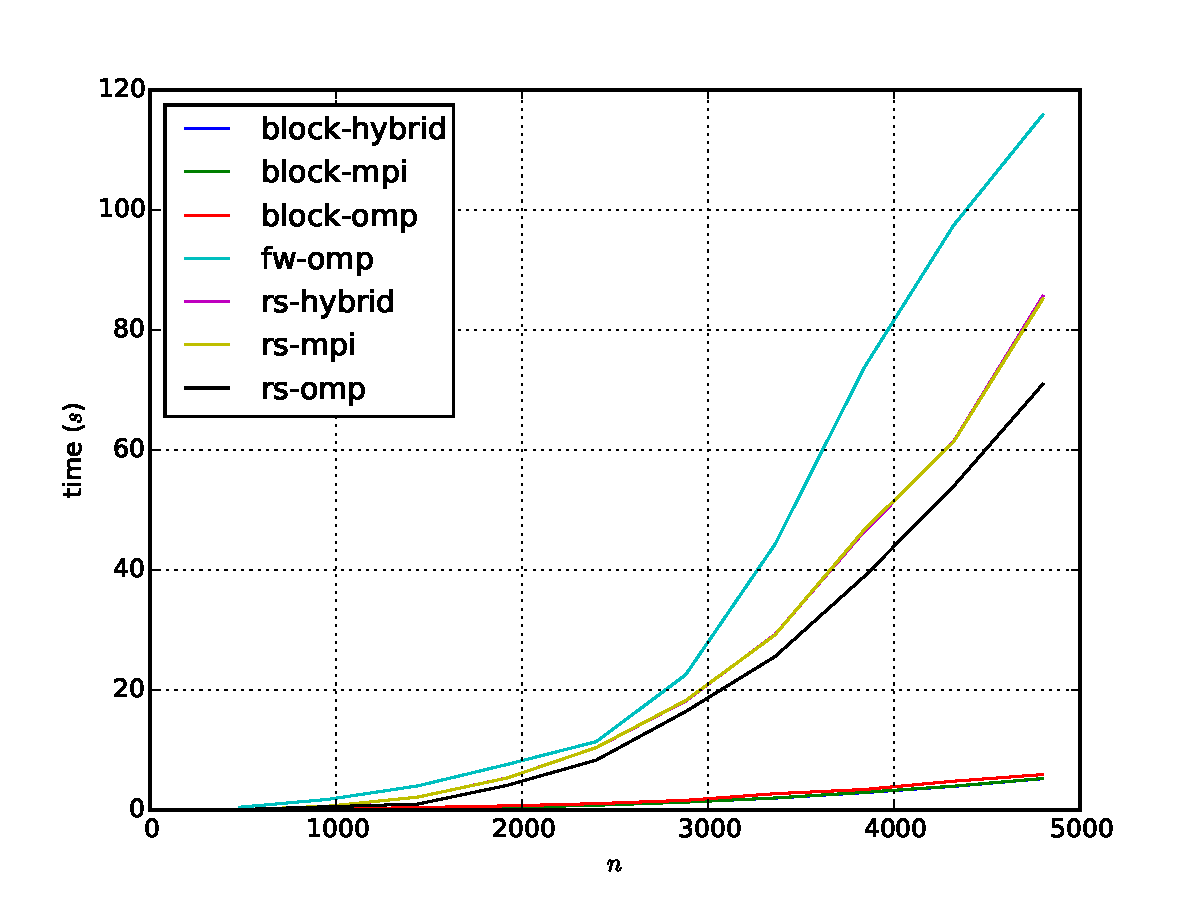
\includegraphics[width=\textwidth]{plots/all.pdf}
  \caption{%
    Performance comparison of all algorithms excluding \fwmpi{} and \fwhybrid{}.
  }
  \label{fig:perf}
\end{figure}
